\chapter{Discussion}

% Start with the big picture.
Our analysis of the Orion A and Orion B molecular clouds reveals a complex interplay between morphology, topology, and star formation activity. 
By combining perimeter–area scaling, Euler characteristic profiles, and mass–size relations, we obtain a consistent picture of how structural complexity varies across column densities and how these variations relate to the presence of young stellar objects.

% Synthesize the fractal dimension results (global and local).
The global fractal dimension is based on the idea that if a structure is self‑similar—i.e., lacks a characteristic scale—its perimeter and area should follow a power‑law scaling, appearing as a straight line in a log–log diagram.  
Turbulence is known to play a key role in organizing structure within molecular clouds, and the perimeter–area method provides a way to quantify how much this self‑similar behavior influences the observed morphology.

Our global perimeter–area analysis reveals distinct structural regimes within Orion~A, with a clear change in slope that reflects different levels of complexity at low and high column densities.  
In contrast, Orion~B maintains a more uniform fractal signature.  
This contrast already begins to suggest that Orion~A and Orion~B are governed by different physical conditions.

For Orion~A, a double fit is required, indicating a change in the underlying physics. The double fit can be seen in Figure \ref{fig:orion_A_global_double_fit}. 
This transition occurs at a column density of \(N = 1.23 \times 10^{22}\,\mathrm{cm}^{-2}\), marking a physically significant scale.  
At this threshold, the structural properties of Orion~A shift, coinciding with the onset of active star formation and the emergence of dense cores \cite{lada2010star}.  
The concurrent changes in fractal dimension and topology at this scale suggest a direct link between the cloud’s morphology and the physical processes driving star formation.

Without applying the double fit, the global fractal dimension is \(D = 1.35 \pm 0.01\). The single fit for Orion A can be seen in Figure \ref{fig:orion_A_global}. 
This value is in good agreement with previously reported fractal dimensions for molecular clouds derived with alternative methods \cite{elmegreen1996fractal}, where typical values are around \(D \sim 1.3\).  
Numerical simulations based on two‑dimensional compressible turbulence in a self‑gravitating ISM also reproduce similar values \cite{1994fns..book..515Y}.  
Note that many studies report the three‑dimensional fractal dimension, which is related to the two‑dimensional value by adding unity.

When the data are separated into two regimes, we obtain \(D = 1.65 \pm 0.01\) at higher column densities and \(D = 0.97 \pm 0.03\) at lower column densities.  
Although a fractal dimension smaller than 1 is not expected in theory, this result is likely influenced by the limited number of data points contributing to the low‑density fit.  
Even so, the trend is informative: a fractal dimension approaching 1 indicates smoother, simpler boundaries, whereas higher column densities exhibit more complex, space‑filling structures.

% to-do: do we see this visually?
With these types of methods, it is important to also consider if our conclusion match what we actually see in the cloud. To this end, we see in the Gallery that: 

Taken together, these results suggest that the processes driving self‑similarity—such as turbulence—become less dominant once dense cores emerge.  
Beyond this threshold, the cloud’s structure deviates from scale‑free behavior, reflecting the impact of star formation on its morphology.

In Orion~B, by contrast, no such break is required.  
This outcome is broadly consistent with expectations, as Orion~B is known to be a more turbulent molecular cloud.  
In such an environment, scale‑free behavior dominates across the column‑density range analyzed, as reflected in the high quality of the single global fractal dimension fit (Figure \ref{fig:orion_B_global}).  
The emergence of cores does not appear to disrupt the hierarchical structuring.  
Together, these findings provide the first elements of a coherent picture described by the Minkowski functionals.

% to-do:do we see this visually?
Again, we need to ask ourselves if visually these conclusions make sense.

It is also instructive to compare these results with measurements obtained for other molecular clouds.  
Studies applying perimeter–area methods or similar techniques have typically found global fractal dimensions in the range \(D \sim 1.2{-}1.4\) for nearby star‑forming regions.  
For example, \cite{falgarone1991hierarchical} reported \(D \approx 1.36\) for CO maps of Perseus and Ophiuchus, while \cite{sanchez2005fractal} found values between 1.25 and 1.35 for a sample of Galactic molecular clouds.  
These values are broadly consistent with the single‑fit results for Orion~A (\(D = 1.35 \pm 0.01\)) and Orion~B (\(D = 1.40 \pm 0.01\)), reinforcing the interpretation that the large‑scale morphology of these clouds is comparable to that of other regions in the Milky Way.

What is less commonly reported, however, is the clear break we observe in Orion~A at \(N = 1.23 \times 10^{22}\,\mathrm{cm}^{-2}\).

Naturally, this method has limitations.  
Numerical errors can arise when calculating perimeters and areas for very small structures at high column densities.  
Straight contours, resulting from limited observational resolution, should also be avoided, as they can distort the scaling relationships on which the method relies.

The local fractal dimension builds on the perimeter–area relation, but in this case the relation is inverted to obtain a proxy for the boundary complexity of individual structures.  
This measure offers a more nuanced view than the global approach, capturing how structural complexity evolves with column density on a local scale.

The local fractal dimension calculated at each column‑density threshold shows a consistent trend toward \(D \approx 2\) at higher thresholds for both Orion~A and Orion~B (Figure \ref{fig:local_Orion_A_B}).  
This behavior appears to arise not from the increasing complexity of individual structures, but rather from the growing, interconnected network of cores, fibers, and filaments that emerge as the cloud fragments at higher column densities.
The average local fractal dimension for both Orion~A and Orion~B is approximately 1.7, which remains within the expected range for molecular clouds. This value suggests that, on average, the boundaries of structures in both regions are moderately complex—more intricate than simple geometric shapes, but not fully space-filling. Such averages are consistent with previous studies and support the interpretation that turbulence and hierarchical fragmentation are key drivers of cloud morphology at these scales.

% to-do: do we see this visually?
% to-do: do the peaks represent something?
Some visual examples are helpful to illustrate this behavior (see Gallery).  
Prominent peaks in the local fractal dimension can be associated to..

Because this approach is less commonly used in studies of molecular clouds, direct observational comparisons in the literature are limited.  
Nevertheless, the trends we identify are consistent with the overall picture painted by the global fractal dimension and align well with our physical understanding of these regions.

The closest analytical work on this topic employs a related framework, the mass–size scaling relation \cite{beattie2019relation}.  
Since mass can be treated as a proxy for area, and size as a proxy for perimeter, this method is conceptually similar to the perimeter–area scaling relation used here.  
In their simulations, they report similar trends in the inferred fractal dimension as a function of Mach number (Figure \ref{fig:beattie_fractal_dimension}).
This comparison demonstrates that the results from our method are supported by independent simulation-based studies and further emphasizes the sensitivity of fractal measures to the turbulent state of the cloud. The uncertainties associated are also similar in magnitude, proving also that our approach is reasonable.

\begin{figure}[t]
    \centering
    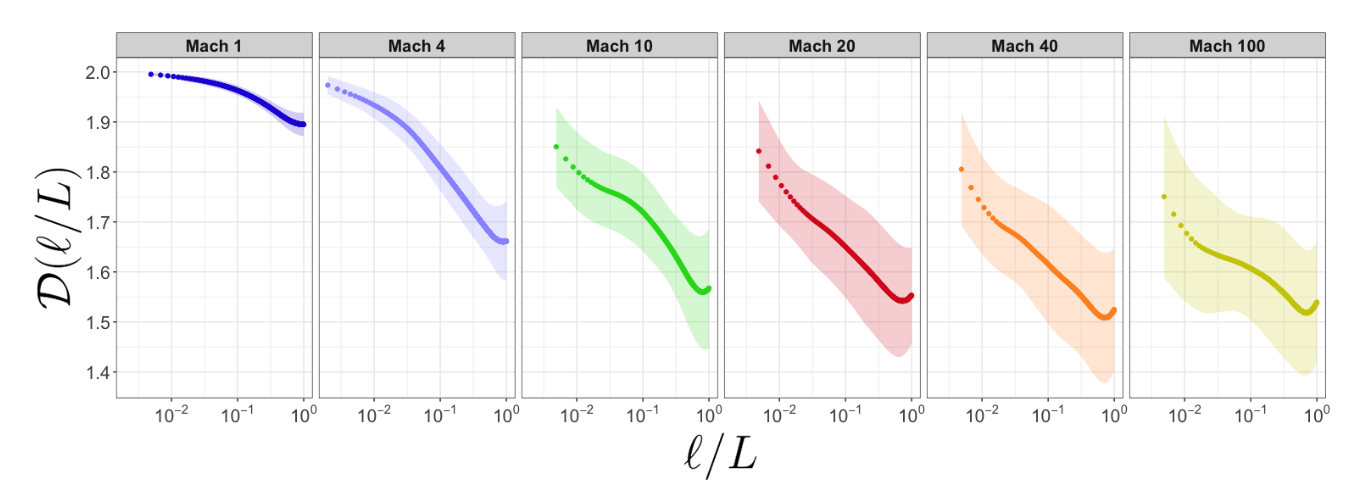
\includegraphics[width=0.75\textwidth]{figures/beattie_fractal_dimension.png}
    \caption{Fractal dimension derived from the mass–size relation as a function of Mach number \cite{beattie2019relation}.  
    Note that the x-axis is inverted relative to our representations above.}
    \label{fig:beattie_fractal_dimension}
\end{figure}

As with the global method, certain limitations must be considered.  
Straight edges introduced by limited angular resolution at low column densities, as well as very small structures at the highest column densities, can affect the measurements.  
For these reasons, the usable column‑density range is narrower than the full range provided by the maps.

% Integrate topological insights (Euler characteristic).
% To-Do:
% Remake Images (after making sure that the definition is correct)
Furthermore, the Euler characteristic highlights clear differences between Orion~A and Orion~B.  
Orion~A exhibits a profile that closely resembles the behavior expected from Gaussian Random Field simulations, with a well-defined peak at approximately \(1.64 \times 10^{22}\,\mathrm{cm}^{-2}\).  
This threshold is significant, echoing the transition seen in the global fractal dimension analysis, and marks the emergence of dense cores within the cloud.

In contrast, Orion~B shows no such pronounced peak, instead displaying a more gradual, almost linear decrease.  
If Orion~B is indeed more strongly influenced by turbulence, this behavior is consistent with a more scale-free, less clustered structure, where the appearance of dense cores is more gradual and widely distributed.  
The topological analysis therefore reinforces the notion that turbulence governs the structural evolution of Orion~B, while Orion~A undergoes distinct transitions closely tied to star-formation thresholds.

% expand these, explain visually some more also connected to the stuff above
Visual examples of the changes in the Euler characteristic for Orion~A and Orion~B are provided in Figures~\ref{fig:Euler_Orion_A} and~\ref{fig:Euler_Orion_B}.

\begin{figure}[t]
    \centering
    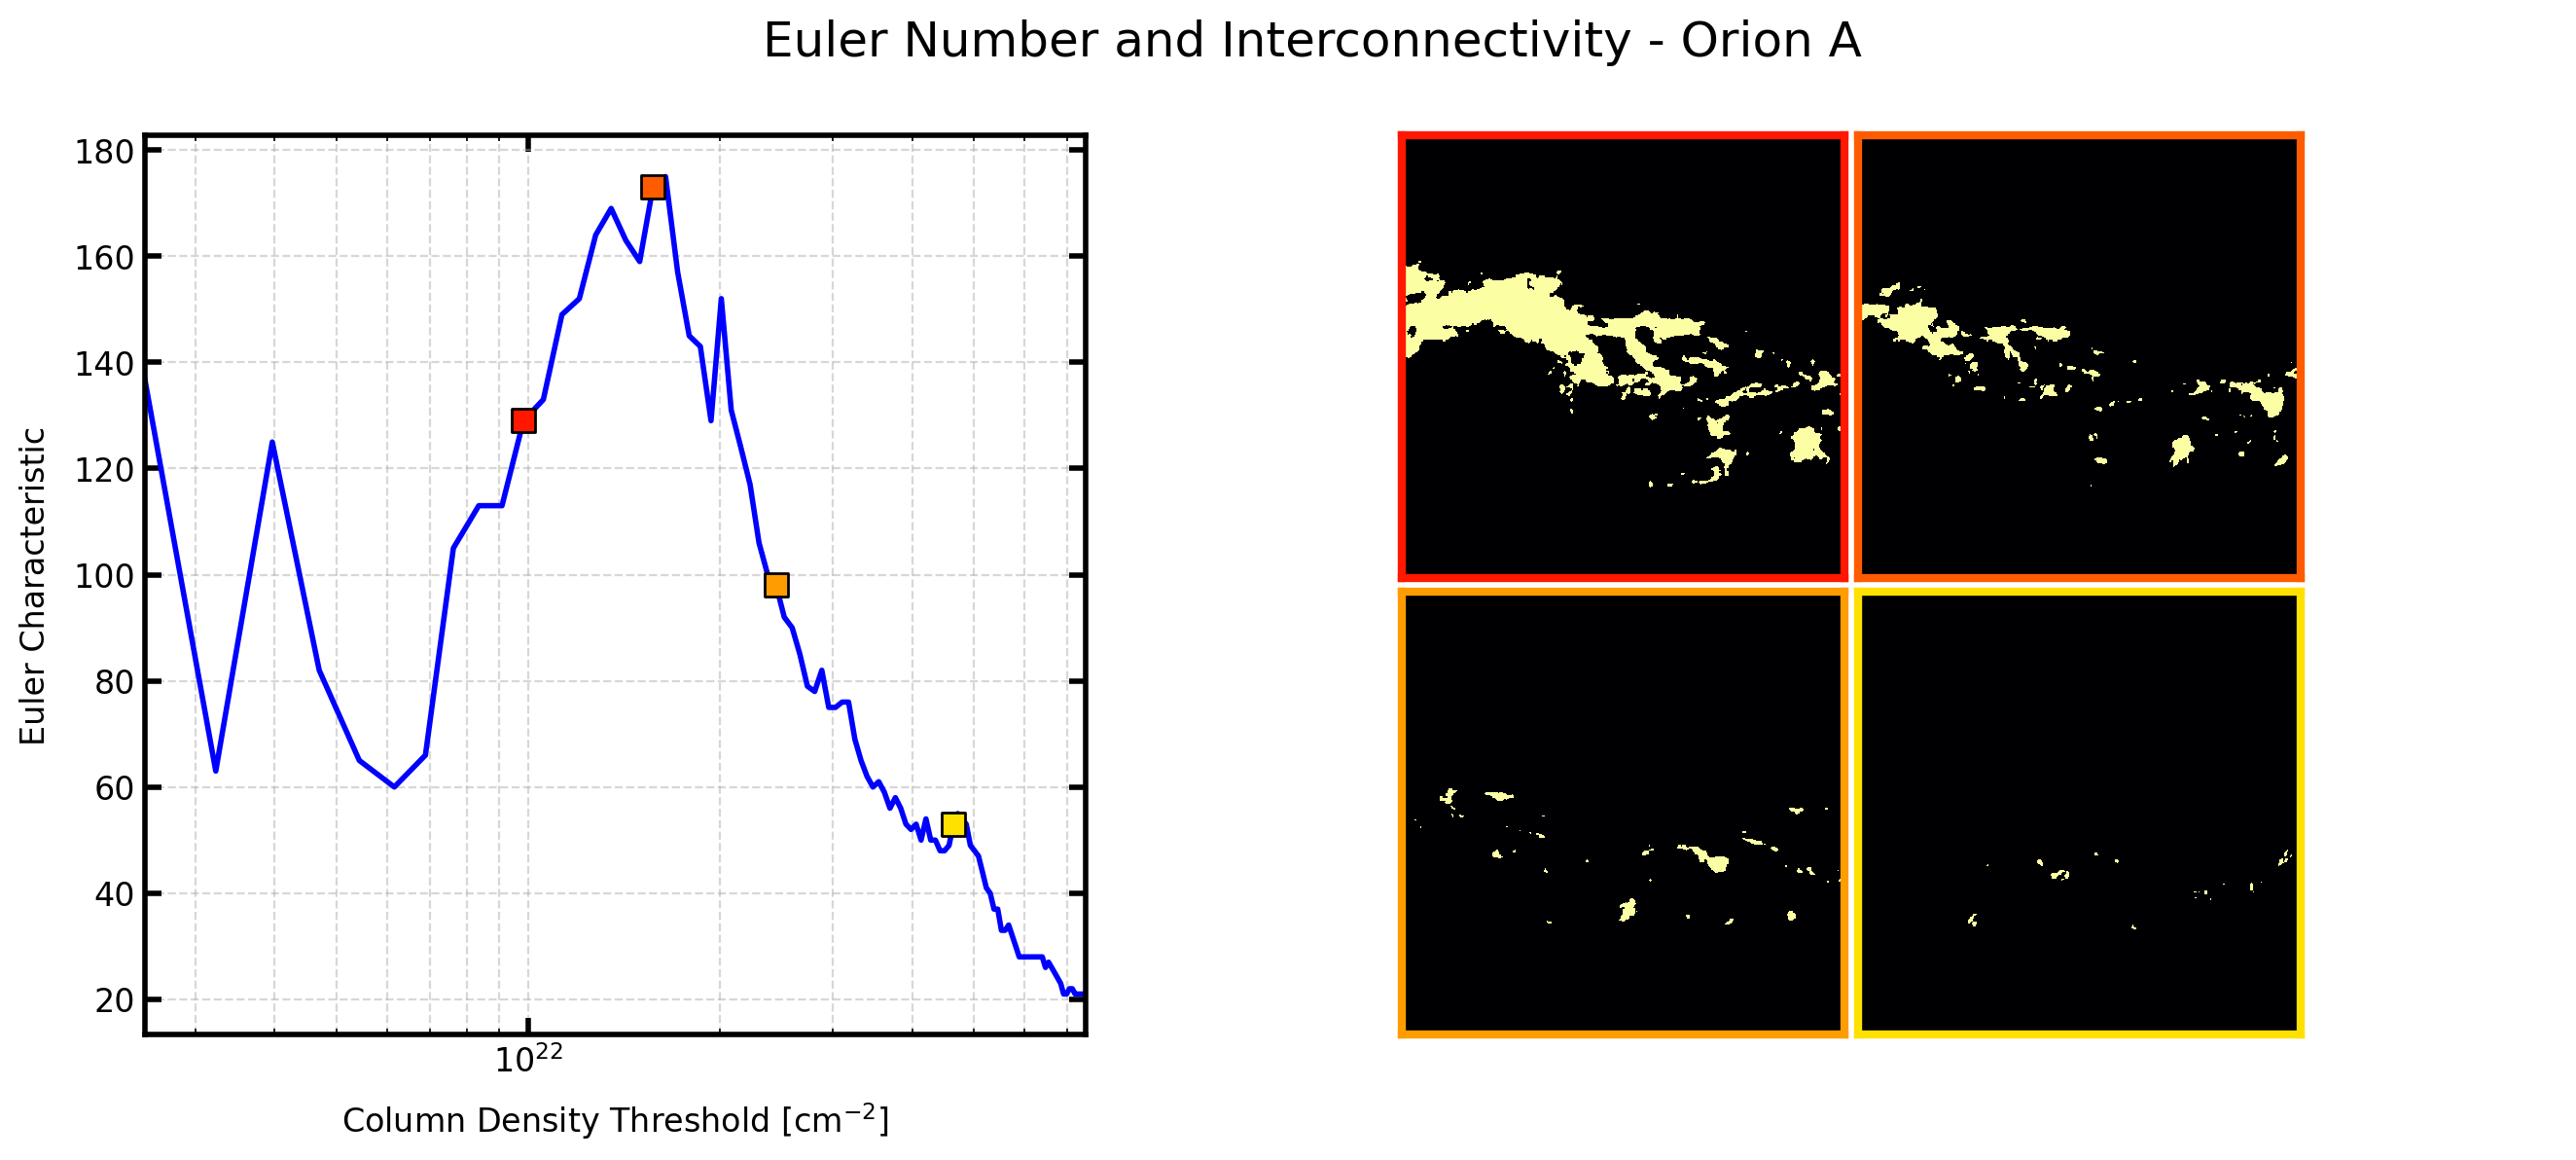
\includegraphics[width=0.65\textwidth]{figures/euler_Orion_A.png}
    \caption{Euler characteristic as a function of column density (left) and four examples of structures (right) marked by colored boxes on the graph (Orion A).}
    \label{fig:Euler_Orion_A}
\end{figure}

\begin{figure}[t]
    \centering
    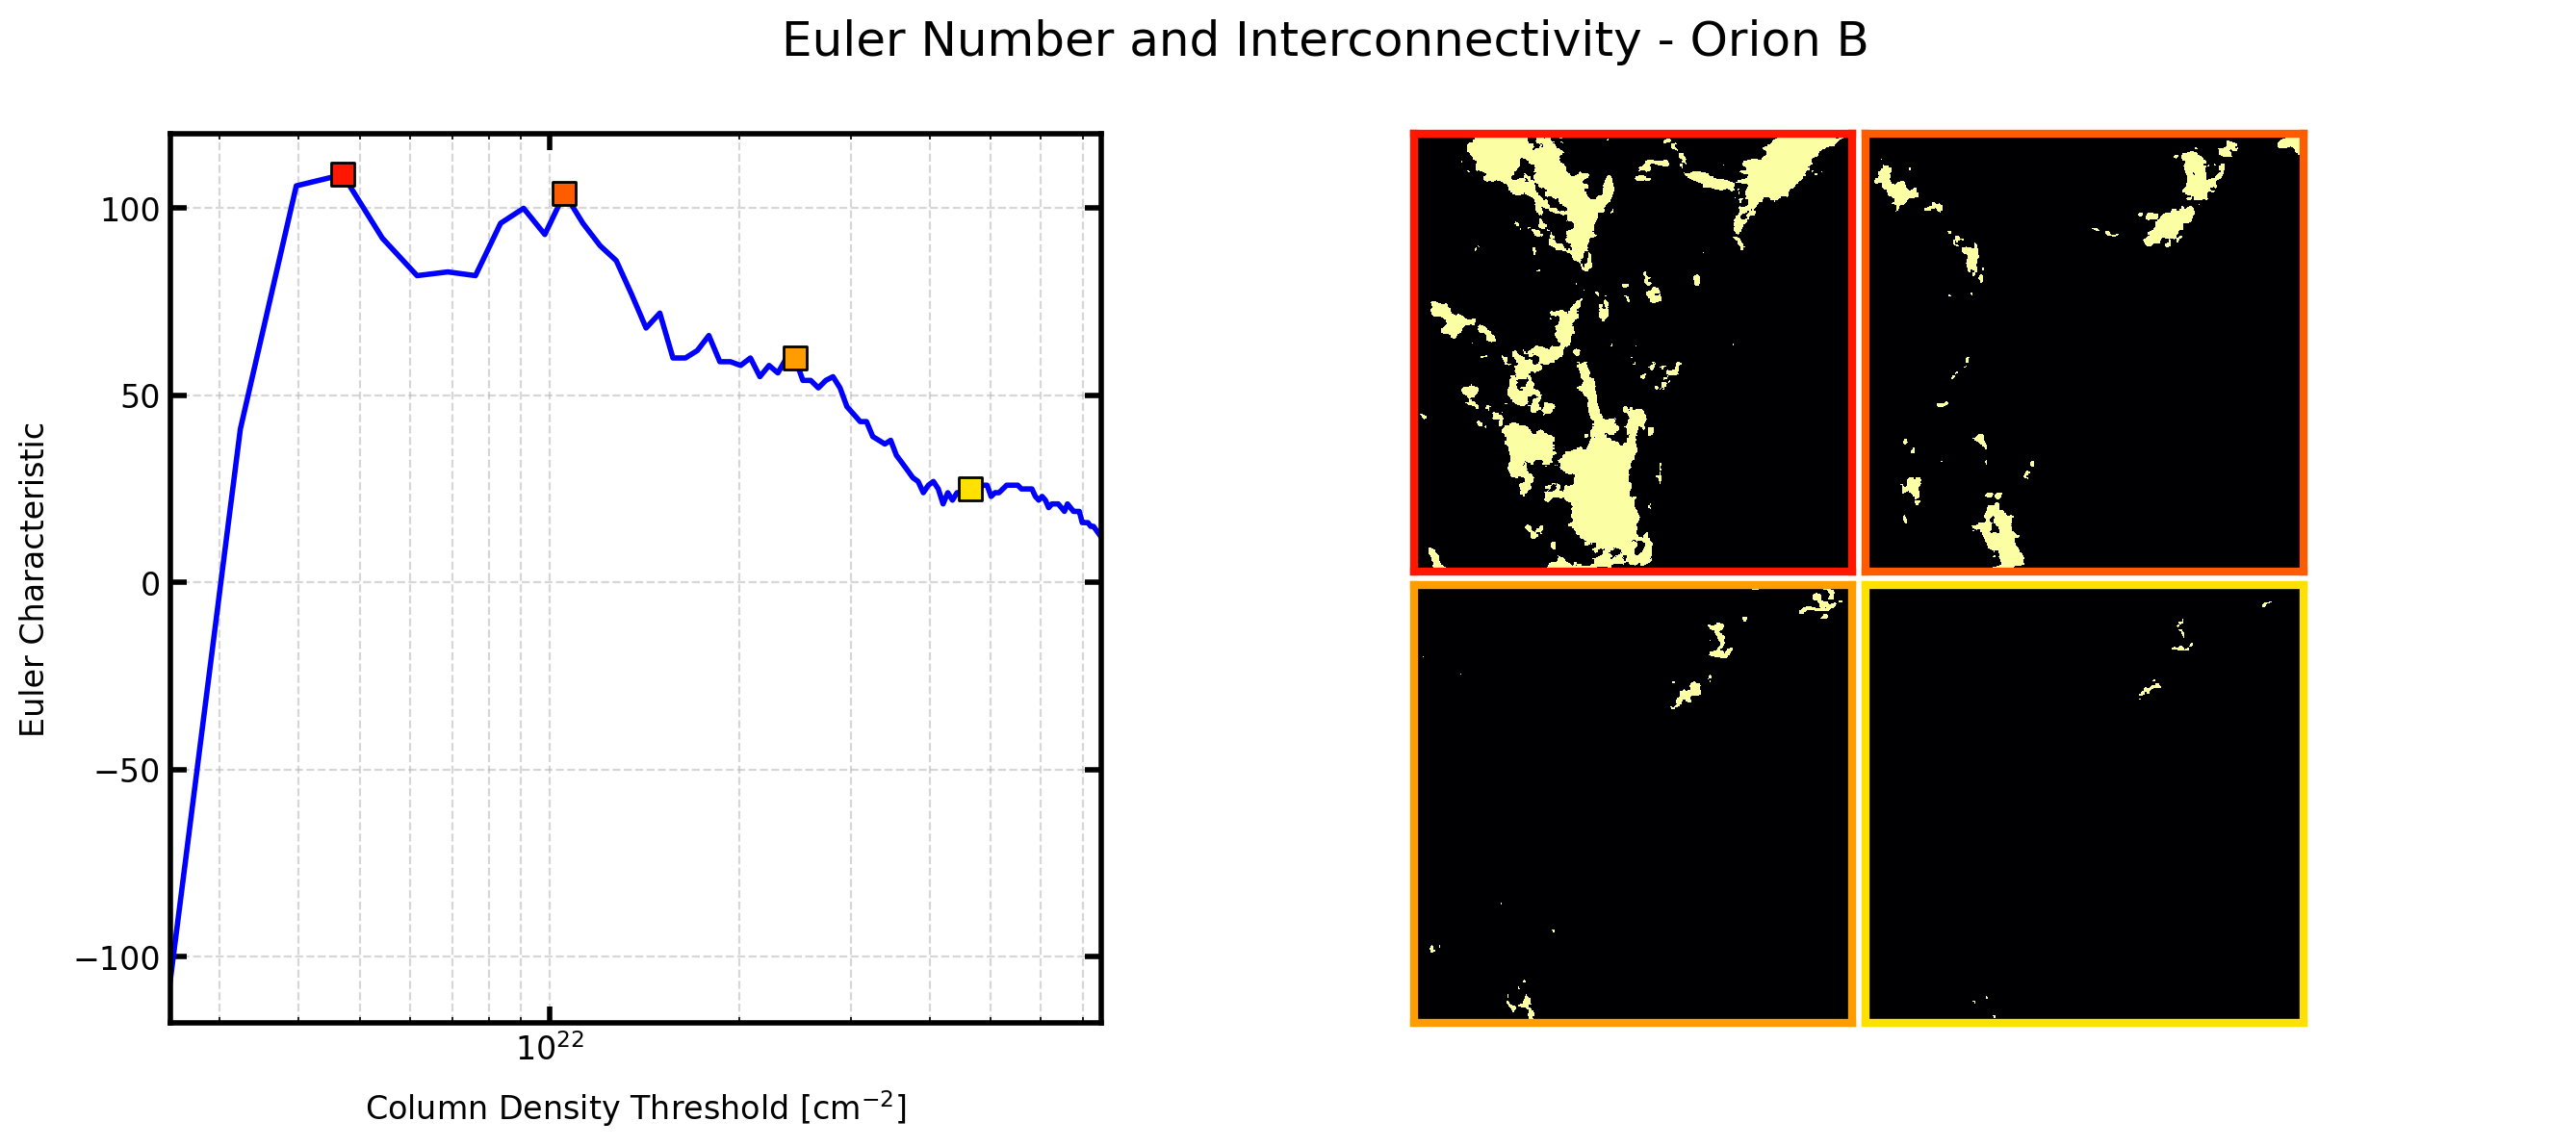
\includegraphics[width=0.65\textwidth]{figures/euler_Orion_B.png}
    \caption{Euler characteristic as a function of column density (left) and four examples of structures (right) marked by colored boxes on the graph (Orion B).}
    \label{fig:Euler_Orion_B}
\end{figure}

% Bring in the MSD plane and individual-structure analysis.
The next step in our analysis was to examine individual structures in the context of the local fractal dimension.  
Using the hierarchical segmentation provided by the dendrogram, we tracked the properties and positions of individual components at each column‑density threshold.

As an initial step, we analyzed how the local fractal dimension of these structures varies with column density.  
We found that the ensemble of structures broadly follows the trend observed for the entire cloud, but with a shallower dependence and greater scatter (Figures~\ref{fig:local_A_single_structures} and~\ref{fig:local_B_single_structures}).  

These results raise interesting questions.  
While the ensemble as a whole tends toward \(D \approx 2\) (indicating increasing boundary complexity), one might expect that individual structures would appear smoother and simpler at higher column densities, rather than more intricate.  
This apparent tension motivates a closer look at how structure fragmentation and connectivity influence the derived fractal dimension.

Connecting the fractal dimension with mass and size properties further confirmed this puzzling picture: the smaller and lighther (core-like) the structures, the more they tend towards higher local fractal dimension (Figures \ref{fig:MSD_orion_A}, \ref{fig:MSD_orion_B}, \ref{fig:MSD_orion_A_B}).

Visually this can also be confirmed:

% Connect to star formation.
% which of the two is forming more stars?

% End with a synthesis.

% Global Fractal Dimension 
% Less so in Orion B, this gives a coherent picture of how the Minkowski functionals can describe the physics of the cloud.

comparison with the M**alpha method

Star Formation: method a bit limited by the number and extent of the objects.